\documentclass[convert={outext=.png}]{standalone}

\usepackage[dvipsnames]{xcolor}
\usepackage{tikz}

\begin{document}

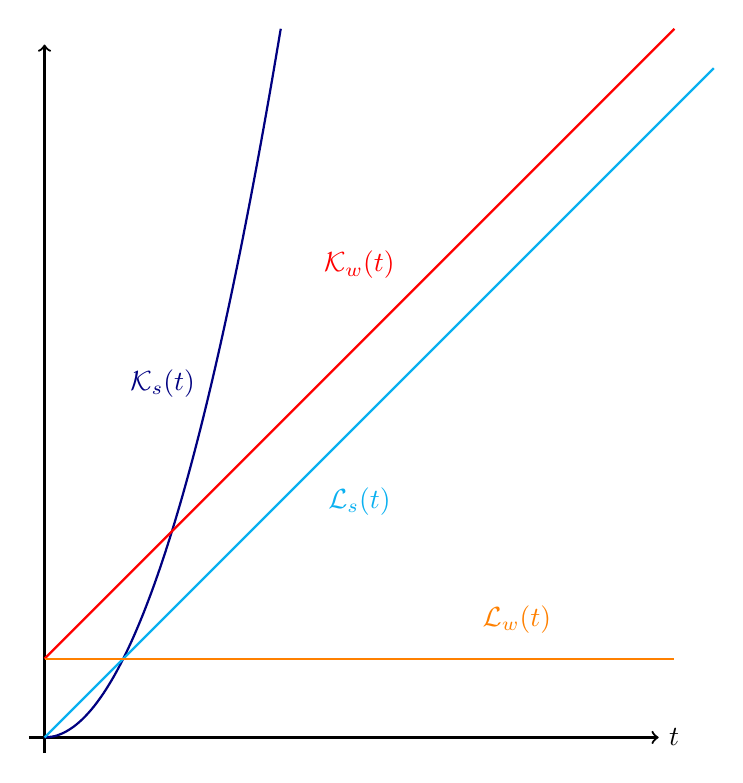
\begin{tikzpicture}[thick]
  % Abscissa
  \draw [->] (-0.2, 0) -- ++(8, 0) node [right] {$t$};

  % Ordinate
  \draw [->] (0, -0.2) -- ++(0, 9);

  % Knowledge of a strong learner.
  \draw [domain=0:3, smooth, NavyBlue] plot (\x, {\x^2});
  \draw (1.5, 4.5) node [NavyBlue] {$\mathcal{K}_s(t)$};

  % Learning of a strong learner.
  \draw [domain=0:8.5, smooth, ProcessBlue] plot (\x, {\x});
  \draw (4, 3) node [ProcessBlue] {$\mathcal{L}_s(t)$};

  % Knowledge of a weak learner.
  \draw [domain=0:8, smooth, Red] plot (\x, {\x + 1});
  \draw (4, 6) node [Red] {$\mathcal{K}_w(t)$};

  % Learning of a weak learner.
  \draw [domain=0:8, orange] plot (\x, {1});
  \draw (6, 1.5) node [orange] {$\mathcal{L}_w(t)$};
\end{tikzpicture}

\end{document}
